\documentclass[a4paper,17pt]{extarticle}
\usepackage{tikz,mathspec,makecell,graphicx,qrcode}
\usepackage[russian]{babel}
\usepackage[top=1cm,bottom=0cm,outer=1.8cm,inner=1.8cm]{geometry}
\parindent=0.6in \parskip=2.8mm

\setmainfont[
	Path = f/,
	BoldFont=lb.ttf,
	ItalicFont=li.ttf,
	BoldItalicFont=lbi.ttf
		]{l.ttf}
\setsansfont[
	Path = f/,
	BoldFont=lb.ttf,
	ItalicFont=li.ttf,
	BoldItalicFont=lbi.ttf
		]{l.ttf}
		
\setmathfont(Digits)[Path = f/]{l.ttf}
\setmathfont(Latin)[Path = f/]{li.ttf}

\begin{document} \thispagestyle{empty}

\begin{center} \begin{tabular}{ccc}
	\makecell[c]{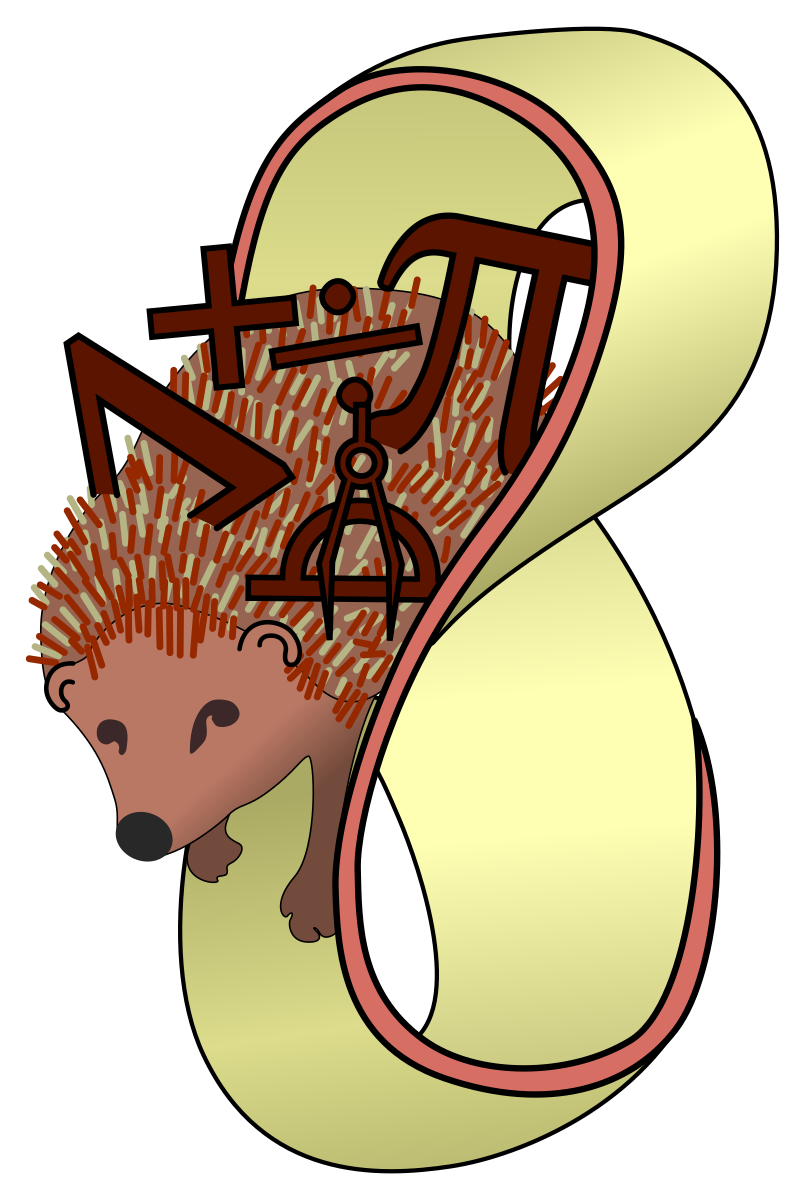
\includegraphics[height=3.7cm]{h}} &
	\hspace{0.7cm} &
	\makecell[c]{
\includegraphics[height=1.75cm]{funds}}
\end{tabular}

\begin{tabular}{l}
	\makecell[l]{{\large\bf 13 марта 2021 года}\\
		{\large\bf мы принимаем олимпиаду}\\
		{\large\bf «Математика НОН-СТОП»}}
\end{tabular}\end{center}

«Математика НОН-СТОП» — уникальная олимпиада, направленная на привлечение интереса школьников не только к олимпиадным задачам как таковым, но и к решению проблем глубокого исследовательского характера. Она является проектом фонда «Время науки», а в 2019–2021 годах проводится при поддержке Фонда президентских грантов. Её принимают более 25 площадок в Санкт-Петербурге и других регионах.

Особенности олимпиады «Математика НОН-СТОП»:\vspace{-6mm}
\begin{itemize} \itemsep=-1.8mm
	\item[–] оригинальные задания;
	\item[–] задачи как для школьников, впервые пробующих себя в олимпиаде, так и для опытных участников;
	\item[–] разделение задач на пункты A, B, C стимулирует думать не только над решениями, но и над стратегией;
	\item[–] профильные задачи моделируют настоящее научное исследование.
\end{itemize}\vspace{-3.5mm}

Информация о вариантах:\vspace{-6mm}
\begin{center} \begin{tabular}{lll}
	4 класс & 6 заданий A, B, C & $2.5$ часа \\
	5 класс & 6 заданий A, B, C & $2.5$ часа \\
	6 класс & 8 заданий A, B, C & $2.75$ часа \\
	7 класс & 9 заданий A, B, C & $3$ часа \\
	8 класс & 10 заданий A, B, C & $3$ часа \\
	7 класс, проф. & 2 исследовательских задачи & $3$ часа \\
	8 класс, проф. & 3 исследовательских задачи & $3$ часа \\
\end{tabular} \end{center}

\begin{center}
	Успейте зарегистрироваться на олимпиаду!\\[0.3cm]
	{\bf\large rs.mathnonstop.ru}
\end{center}

\tikz[remember picture,overlay]{
	\node[opacity=0.28,inner sep=0pt] at (current page.center)
	{
\includegraphics[width=\paperwidth,height=\paperheight]{h-page}};
}
\clearpage

\end{document}